\documentclass[10pt,a4paper]{article}
\usepackage[margin=14mm]{geometry}
\usepackage{graphicx,booktabs,array}
\setlength{\parindent}{0pt}
\begin{document}
\begin{center}
{\large\bfseries CIGS 0279: scalar multiplier sweep for C60}\par
\vspace{1mm}
{\small 20\% Hadamard sampling; NPL-default noise; one fixed measurement; 512 PDHG iterations}\par
\end{center}

We predicted the positive C60 parameter map once, then reconstructed using
$\Lambda_{\rho}=\rho\Lambda_{\mathrm{C60}}$ for
$\rho\in\{0.1,0.2,\ldots,10.0\}$ (100 runs).
We selected $\rho^*=1.1$ by the largest PSNR on the ground truth.
This is an \textbf{oracle test-image experiment}, not an unbiased test score.

\vspace{2mm}
\begin{center}
\begin{tabular}{lrrrr}
\toprule
Method & PSNR (dB) & SSIM & HaarPSI & MSE \\
\midrule
Zero-filled & 26.513 & 0.5039 & 0.6453 & 2.232e-03 \\
Scalar TV oracle 512 & 33.514 & 0.9173 & 0.8294 & 4.453e-04 \\
C60 rho=1 & 33.422 & 0.9372 & 0.8287 & 4.548e-04 \\
C60 rho=1.1 & 33.454 & 0.9357 & 0.8208 & 4.515e-04 \\
\bottomrule
\end{tabular}
\end{center}
\vspace{-3mm}
\begin{center}
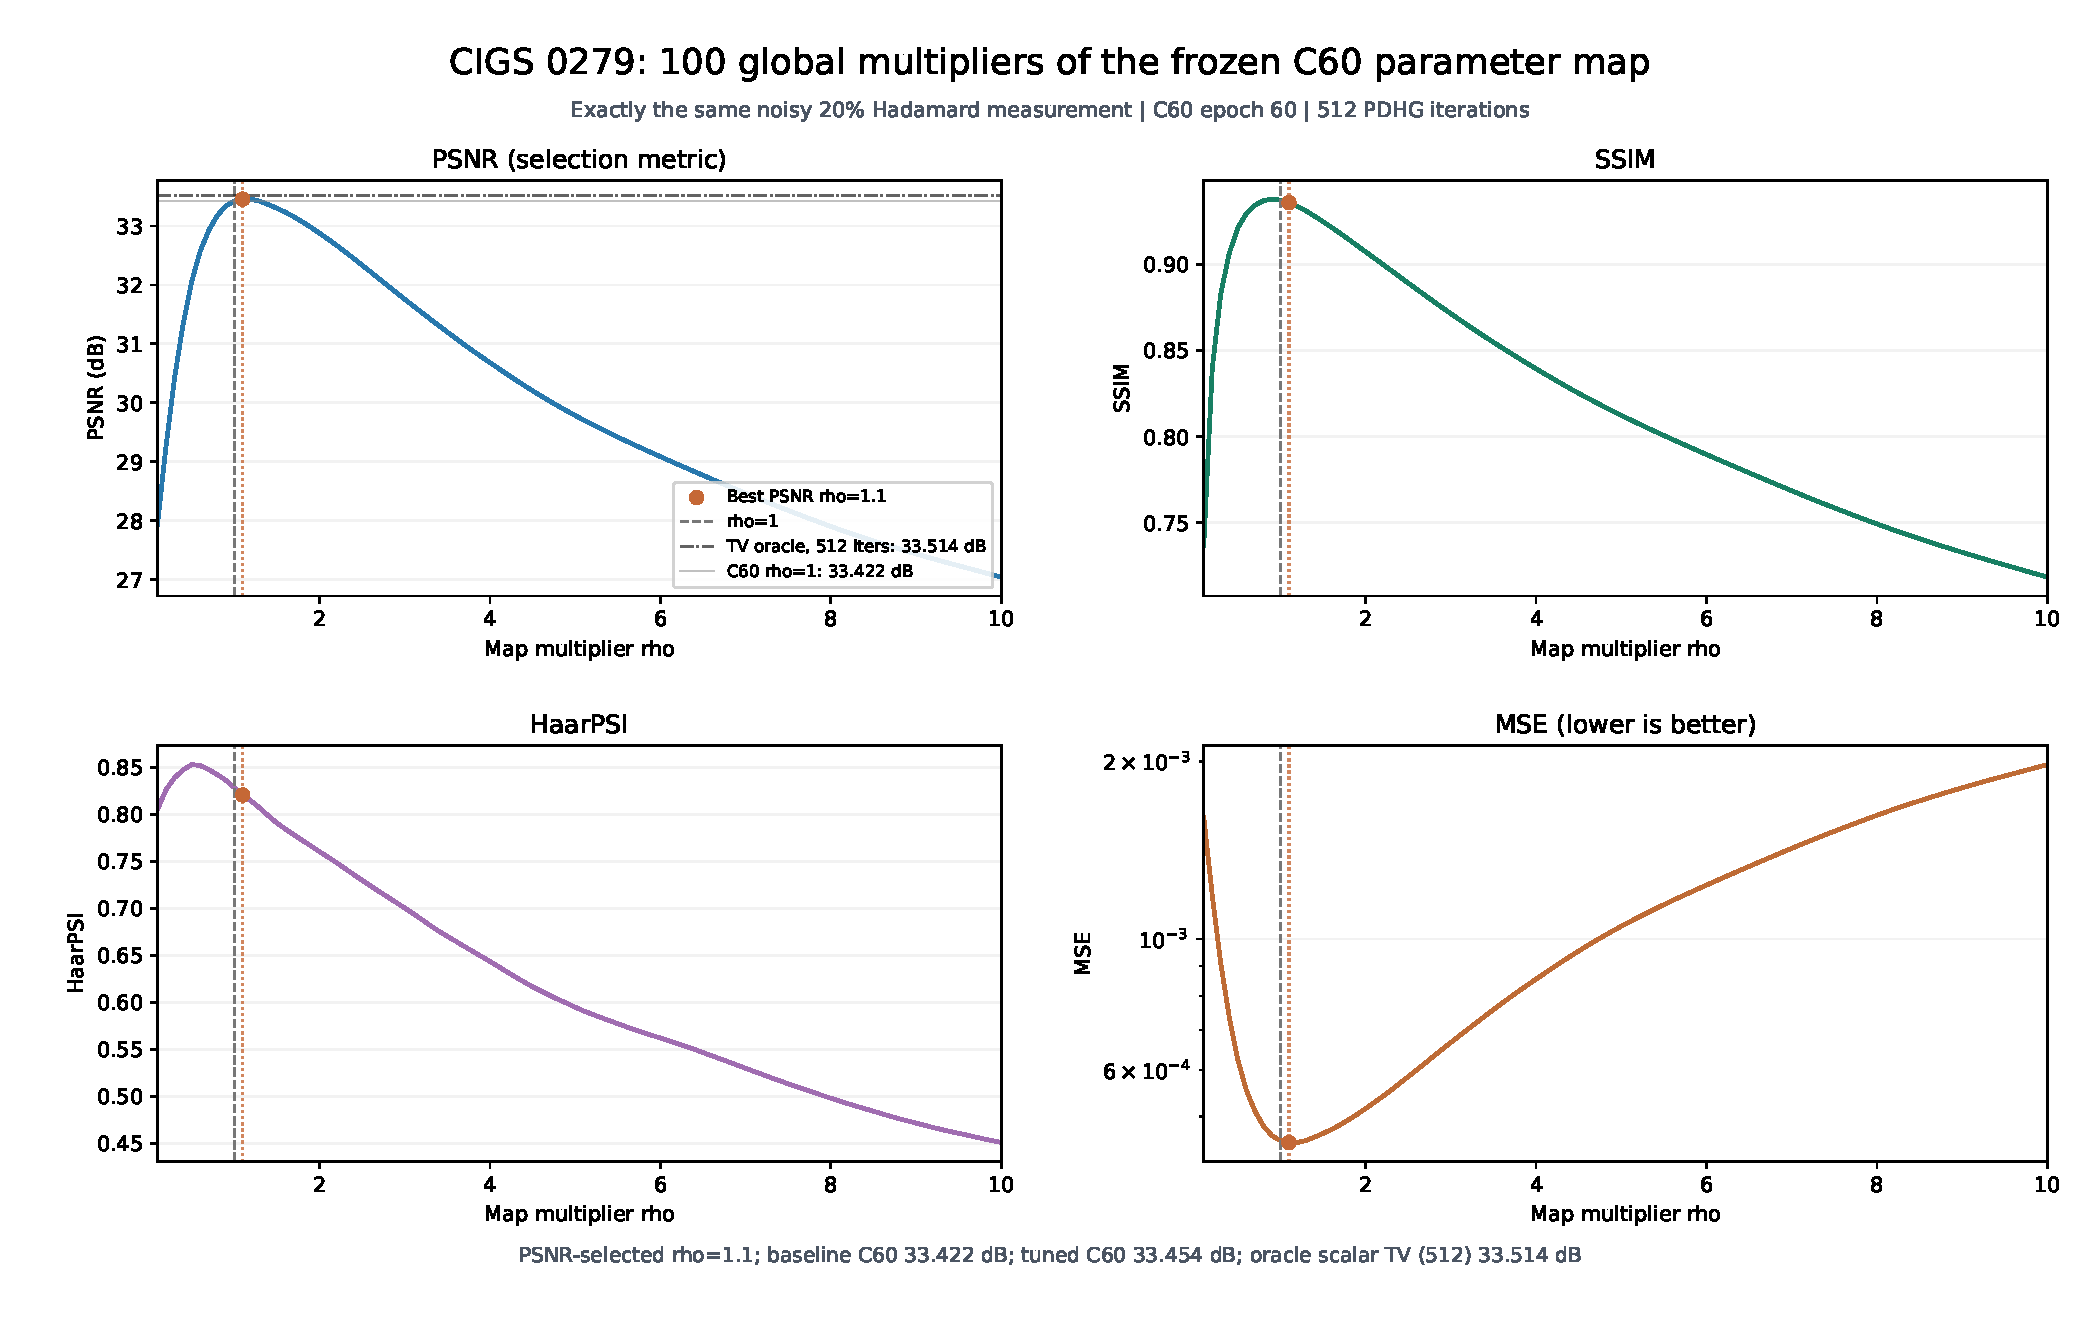
\includegraphics[width=.94\linewidth]{figures/rho_metrics.pdf}\\[-1mm]
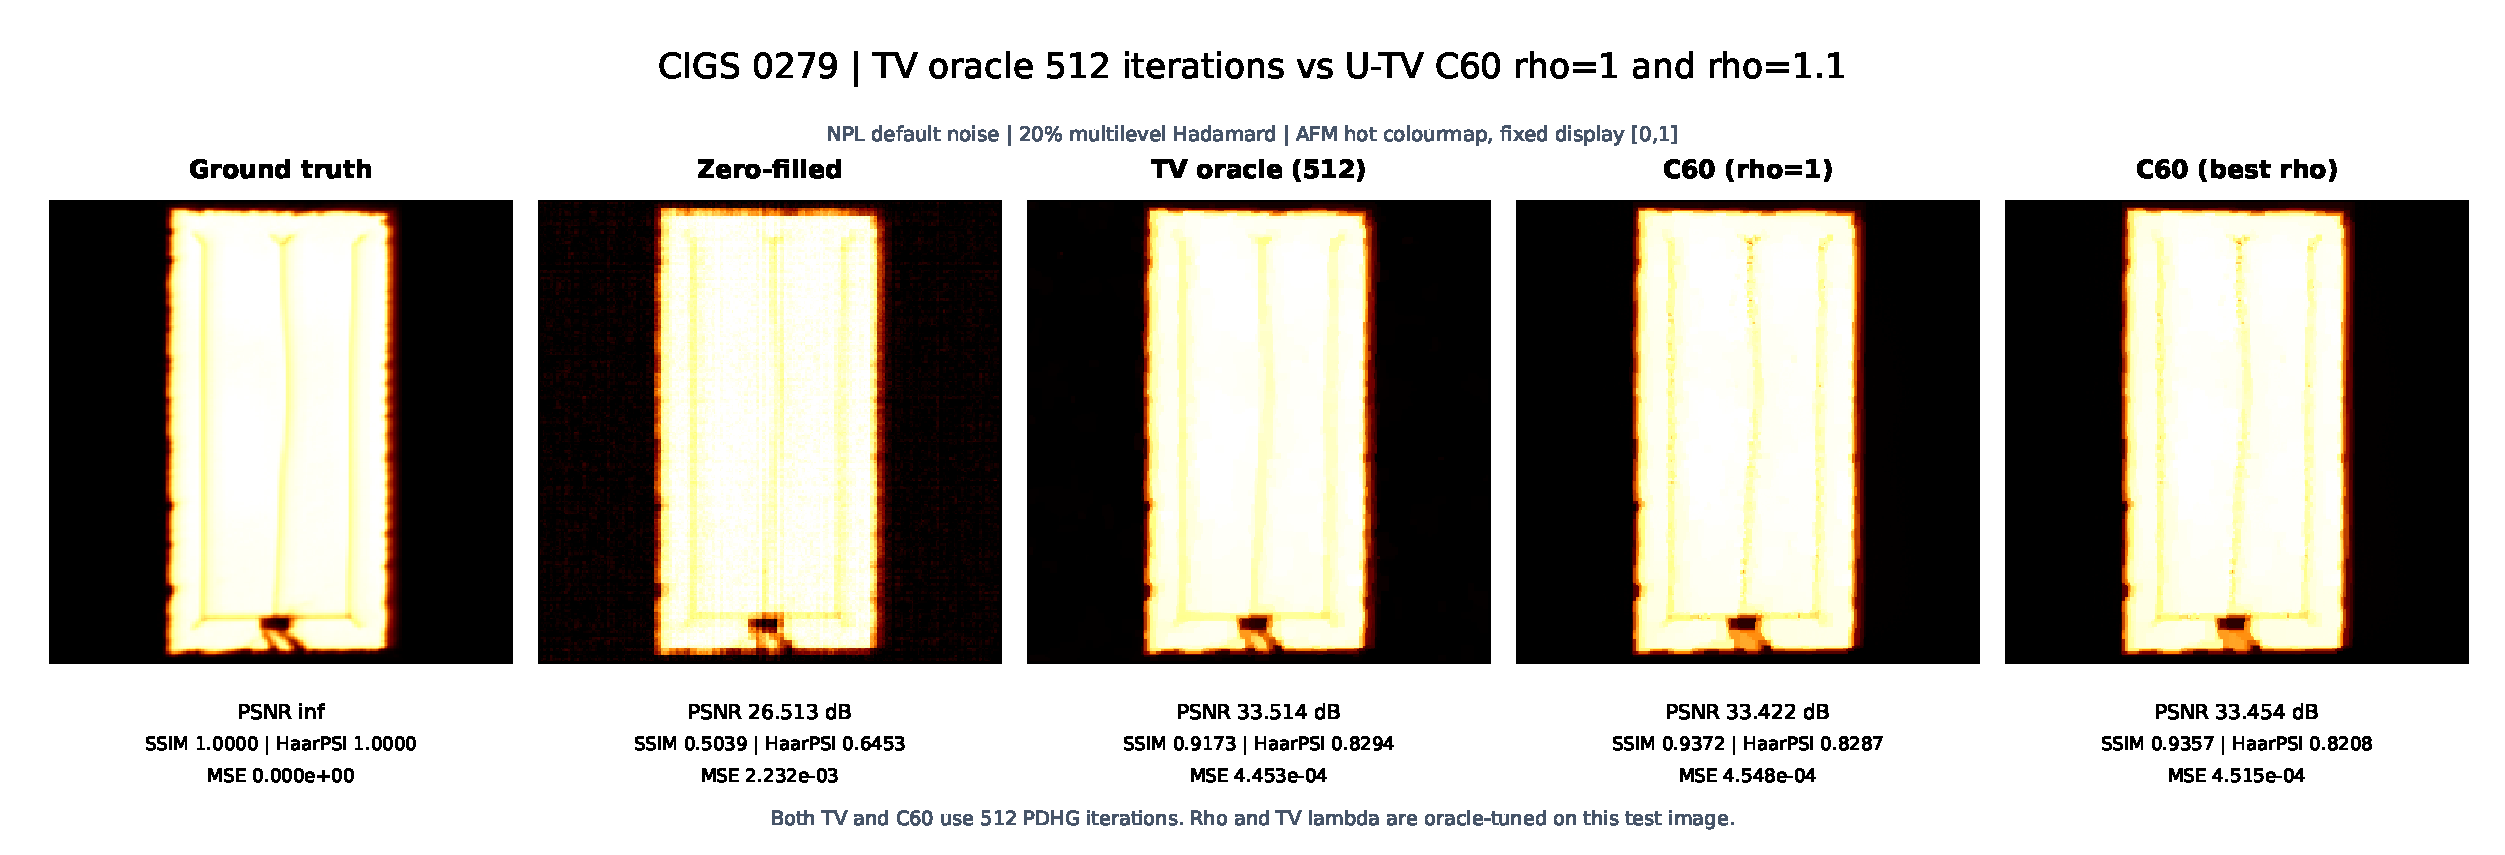
\includegraphics[width=.94\linewidth]{figures/comparison.pdf}
\end{center}
\end{document}
